\FloatBarrier
\subsection{Engine Replacement MDP: Learning the Engine's Transitions}
\label{engine:ch12}

\begin{table}[H]
\centering
\small
\caption{Learning the four Engine Replacement MDP transition rows. Value errors, bounds, and standard errors use two hundred fixed seeds.}
\label{tab:engine_model_learning}
\begin{tabular}{rrrrrr}
\hline
$N$ & mean kernel error & value error & s.e. & simulation bound & s.e. \\
\hline
25 & 0.1556 & 0.5015 & 0.0257 & 14.0040 & 0.7085 \\
50 & 0.1028 & 0.3284 & 0.0168 & 9.2520 & 0.4764 \\
100 & 0.0756 & 0.2435 & 0.0143 & 6.8040 & 0.3902 \\
250 & 0.0502 & 0.1615 & 0.0087 & 4.5144 & 0.2407 \\
500 & 0.0355 & 0.1138 & 0.0060 & 3.1950 & 0.1688 \\
1,000 & 0.0259 & 0.0830 & 0.0045 & 2.3265 & 0.1276 \\
2,500 & 0.0165 & 0.0529 & 0.0030 & 1.4821 & 0.0831 \\
5,000 & 0.0113 & 0.0362 & 0.0021 & 1.0154 & 0.0581 \\
\hline
\multicolumn{6}{l}{Final mean estimates of $P(\mathrm{high}\mid s,a)$} \\
\hline
low, keep & low, replace & high, keep & high, replace & \multicolumn{2}{c}{optimal-policy matches} \\
\hline
0.4998 & 0.0000 & 1.0000 & 0.0000 & \multicolumn{2}{c}{1.000} \\
\hline
\end{tabular}
\end{table}


\begin{figure}[H]
\centering
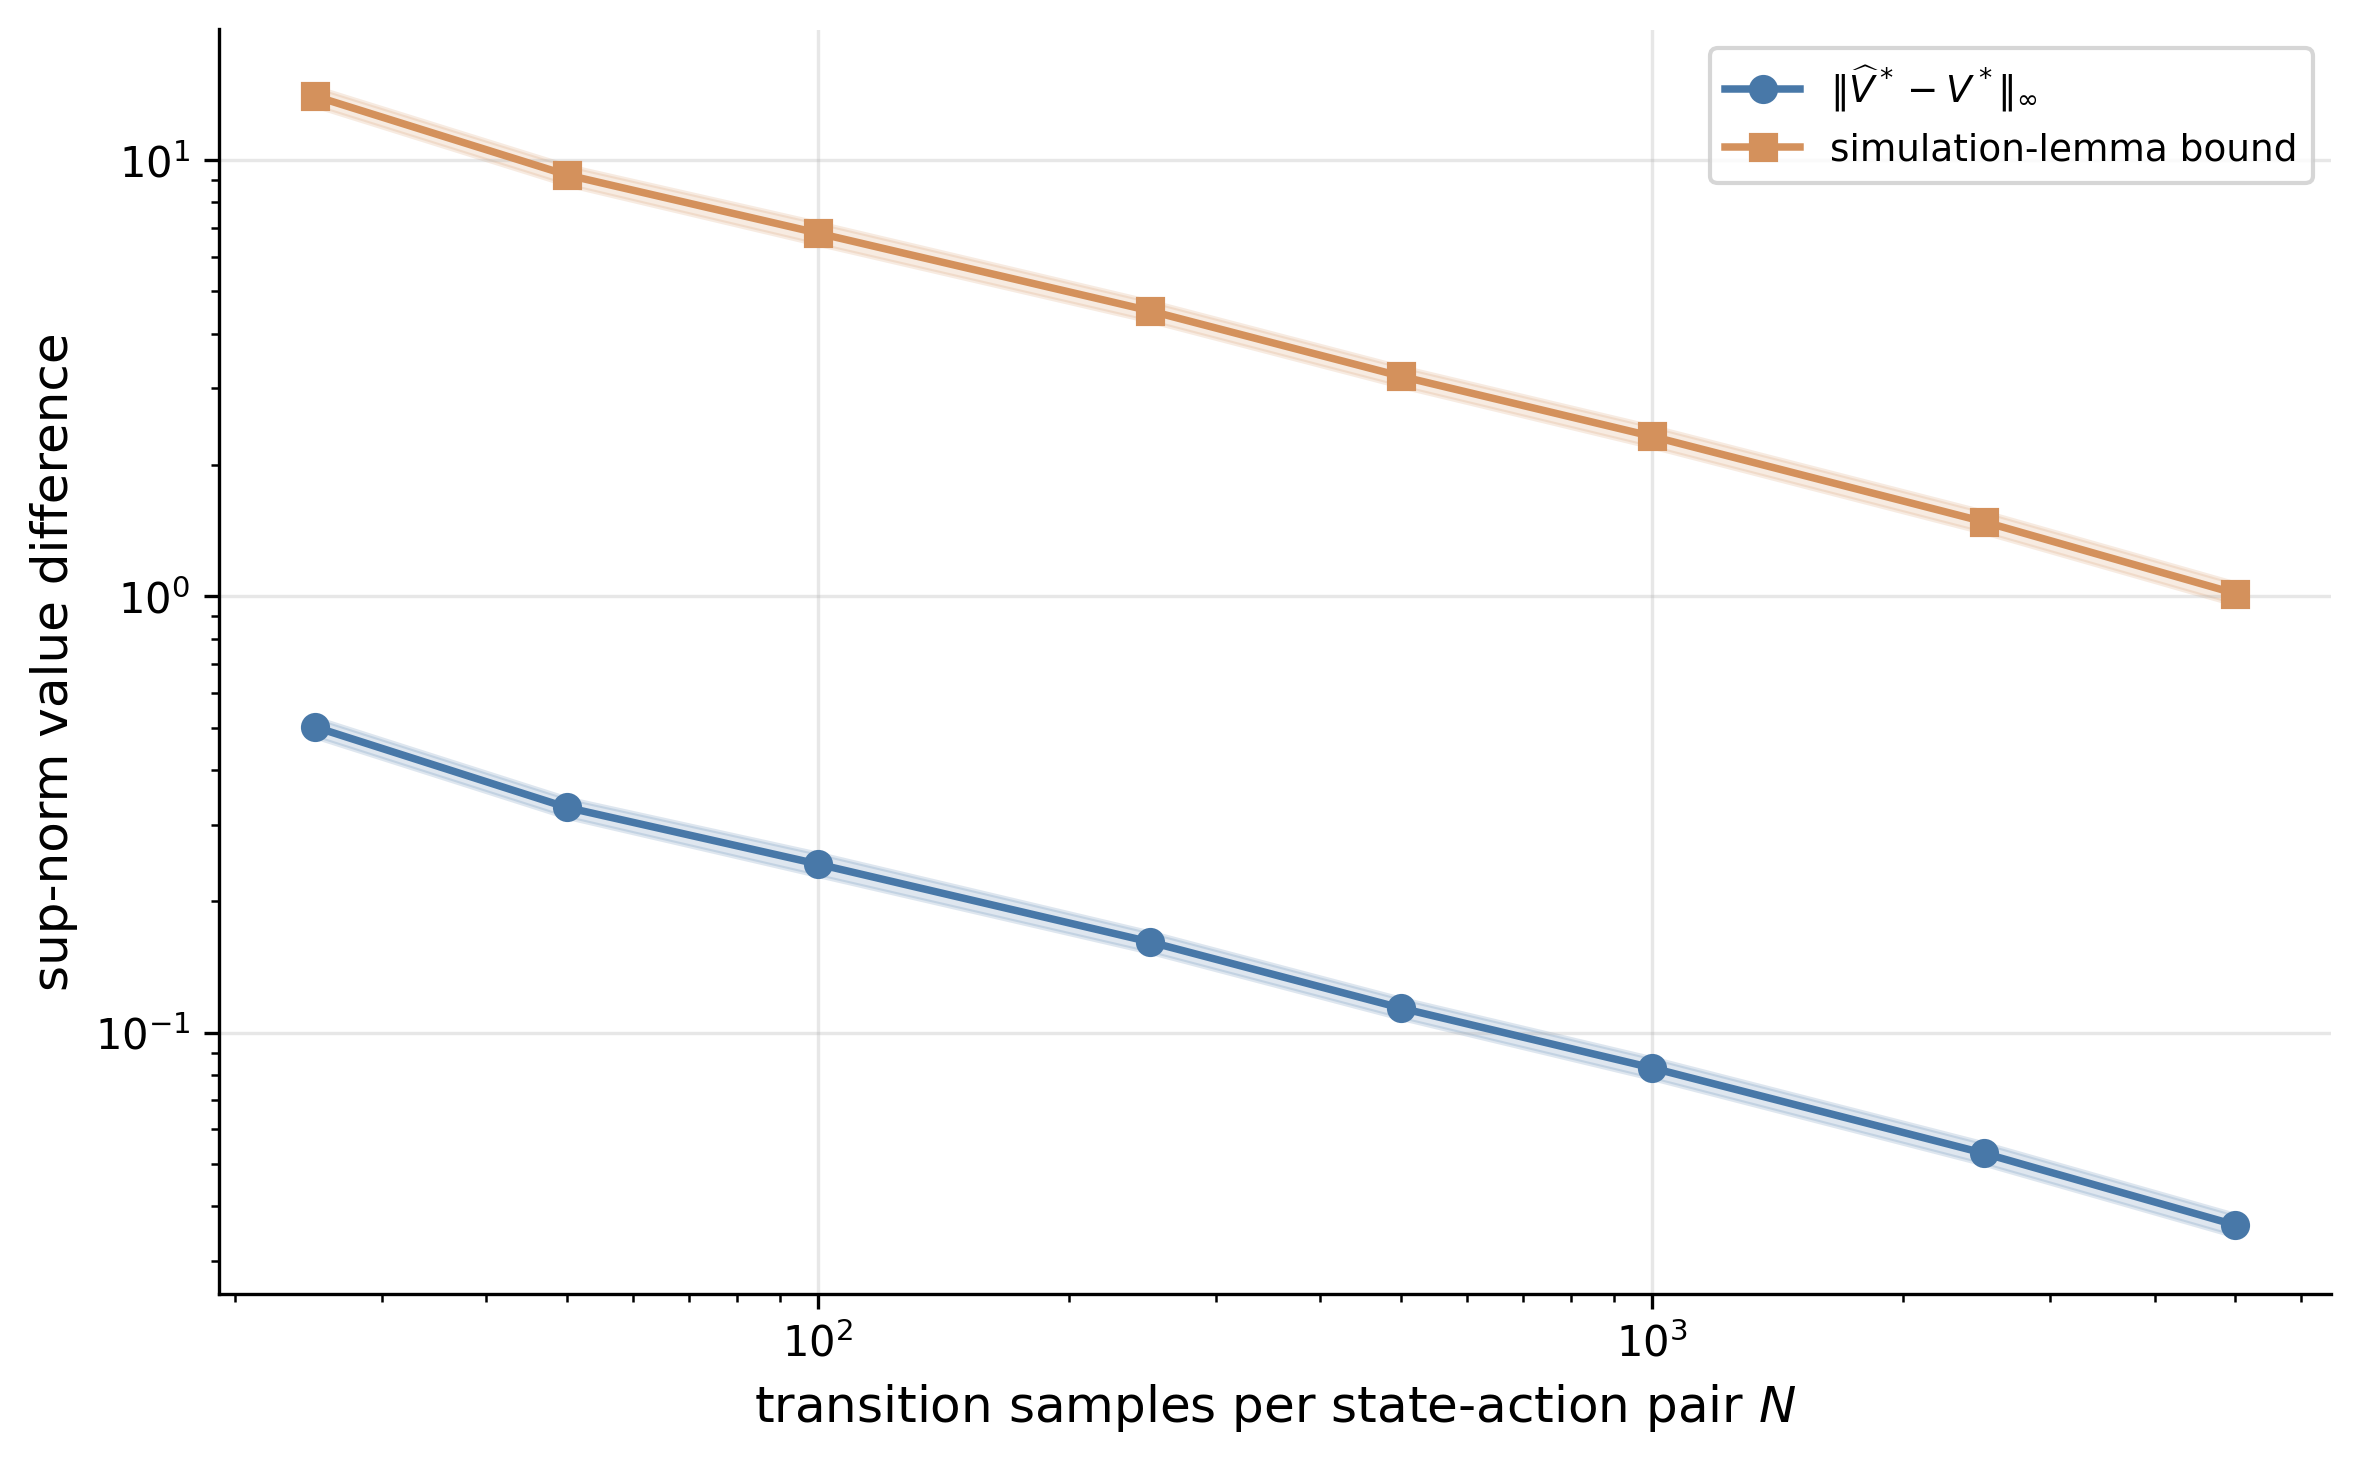
\includegraphics[width=0.72\textwidth]{../ch12_world_models/sims/engine_model_learning.png}
\caption{Optimal-value error and its simulation-lemma bound against transition samples per state-action pair. Lines show means and shaded regions show one standard error over two hundred fixed seeds.}
\label{fig:engine_model_learning}
\end{figure}

For each sample size $N$, the empirical model estimates the probability of a high-mileage successor separately for all four state-action pairs and solves its Bellman optimality equation. Let $\epsilon_P=\max_{s,a}\|\widehat P(\cdot\mid s,a)-P(\cdot\mid s,a)\|_1$. Since rewards are unchanged and $R_{\max}=1$, the discounted simulation lemma gives
\[
\|\widehat V^\star-V^\star\|_\infty
\leq \frac{\gamma R_{\max}}{(1-\gamma)^2}\epsilon_P.
\]
The inequality links transition-estimation error to optimal-value error, and the simulation measures both sides.
Every one of the $1{,}600$ fitted models satisfies this inequality. Three transition rows are deterministic in this example, so their empirical probabilities equal their population values at every $N$. Sampling error enters through the low-mileage keep transition.

Table~\ref{tab:engine_model_learning} and Figure~\ref{fig:engine_model_learning} show that the mean value error falls from $0.5015$ at $N=25$ to $0.0362$ at $N=5{,}000$. The mean bound falls from $14.0040$ to $1.0154$. Both log-log slopes equal $-0.484$, close to the $-0.5$ parametric sampling rate for estimating the Bernoulli transition probability. The empirical optimal policy equals the true keep-then-replace policy in every replication, so the experiment separates value calibration error from policy regret.
\FloatBarrier
